\documentclass[10pt]{beamer}
\usetheme{Boadilla}
\usecolortheme{beaver}
\usepackage[utf8]{inputenc}
\usepackage[english]{babel}
\usepackage{amsmath}
\usepackage{amsfonts}
\usepackage{amssymb}
\usepackage{graphicx}
\usepackage{listings}
\usepackage{multicol}
\usepackage[font=small,labelfont=bf]{caption}
\title{Current state of GCC support for PPU}
%\setbeamercovered{transparent} 
\setbeamertemplate{navigation symbols}{} 
\setbeamertemplate{caption}[numbered]
\author{Arthur Heimbrecht}
%\logo{} 
%\institute{} 
\date{\today} 
%\subject{} 
\begin{document}

\begin{frame}
\titlepage
\end{frame}

\begin{frame}
\tableofcontents
\end{frame}

\section{Basic compiling structure}
\begin{frame}{Basic compiling structure}{Basic compiler structure}
	\begin{columns}
		\begin{column}{0.25\textwidth}
      		\begin{block}{Front-end}
       			\begin{itemize}
       				\item recognizes language
       				\item pre-processing
       				\item type checking
       				\item genreates Immediate Representation
       			\end{itemize}
      		\end{block}
    	\end{column}
    	\begin{column}{0.25\textwidth}
      		\begin{block}{Middle-end}
       			\begin{itemize}
       				\item general optimizations to IR
       				\item ``compiler magic''
       				\item passes IR
       			\end{itemize}
      		\end{block}
    	\end{column}
    	\begin{column}{0.25\textwidth}
      		\begin{block}{Back-end}
       			\begin{itemize}
       				\item target specific
       				\item further/final optimization
       				\item register allocation (spilling)
       				\item generates assembly code
       			\end{itemize}
      		\end{block}
    	\end{column}
    \end{columns}
\end{frame}

\begin{frame}{Basic compiling structure}{Assembler and Linker}
    \begin{block}{Assembler}
       	\begin{itemize}
		\item relative memory handling (notes)
		\item resolving references
		\item generates object files
       	\end{itemize}
    \end{block}
    \begin{block}{Linker}
	\begin{itemize}
       		\item absolute memory handling
       		\item links object files and references
       		\item $\rightarrow$ machine instructions
       	\end{itemize}
    \end{block}
\end{frame}

\begin{frame}[fragile]{Compiler backend}{Key points}
	\begin{itemize}
		\item target files: target.h, target.md, target.c
		\item important ``variables''
			\begin{itemize}
				\item register\_types, \_numbers, \_names
				\item wordsize
				\item basic insns
				\item constraints ('r', 'm'...)
			\end{itemize}
		\item PPU characteristics:
			\begin{itemize}
				\item Power ISA
				\item 32 general registers (32-bit) and 32 vector registers (128-bit)
				\item additional synram
			\end{itemize}
 	\end{itemize}
\end{frame}

\begin{frame}
	\begin{figure}
		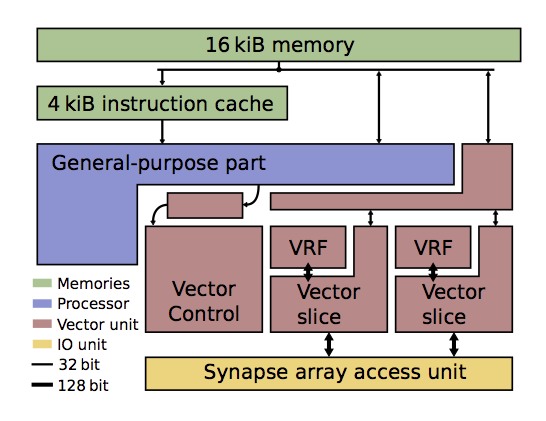
\includegraphics[scale=0.8]{Fig11.png} 
		\caption{Schematic PPU structure, Friedmann et al. "Demonstrating Hybrid Learning in a Flexible Neuromorphic Hardware System", p.7 fig.10, Universität Heidelberg, 2016} \label{fig:PPU}
	\end{figure}
\end{frame}

\section{PPU programming until now}
\begin{frame}[fragile]{PPU programming until now}
	\begin{columns}[t]
		\begin{column}{0.35\textwidth}
    		\begin{itemize}
				\item binutils patch + fxv.h
					\begin{itemize}
						\item close to actual assembly
						\item efficient execution
					\end{itemize}
				\item not user-friendly
				\item reaccuring code
			\end{itemize}    
    	\end{column}    
    	\begin{column}{0.27\textwidth}
     		\begin{block}{code}
        		\begin{lstlisting}[language=C++,basicstyle=\ttfamily\scriptsize,keywordstyle=\color{red}]
				fxv_array_t v1,v2,v3;
				fxv_splatb (1,1);
				fxv_store (&v1, 1);
				fxv_splatb (2,2);
				fxv_store (&v2, 2);
				fxv_add 	(0,1,2);
				fxv_store (&v3, 0);				
				\end{lstlisting}
      		\end{block}
    	\end{column}
    	\begin{column}{0.30\textwidth}
    		\begin{block}{machine instructions}
       			\begin{lstlisting}[language=C++,basicstyle=\ttfamily\scriptsize,keywordstyle=\color{red}]
				28: li        r9,257
				2c: fxvsplath 1,r9
				30: addi      r9,r31,8
				34: fxvstax   1,0,r9
				38: li        r9,514
				3c: fxvsplath 2,r9
				40: addi      r9,r31,12
				44: fxvstax   2,0,r9
				48: fxvaddbm  0,1,2
				4c: addi      r9,r31,16
				50: fxvstax   0,0,r9
			\end{lstlisting}
      		\end{block}
		\end{column}
	\end{columns}
\end{frame}

\section{Current state of PPU backend}
\begin{frame}{Current state of PPU backend}
	\begin{itemize}
		\item start with rs/6000 back-end
		\item add header files and command line option -ms2pp
		\item add s2pp register type $\rightarrow$ overloaded float regs
			\begin{itemize}
				\item needed own internal vector type, bit-masks,...
				\item AltiVec as blueprint
				\item a lot of trouble
			\end{itemize}
		\item basic insns
		\item support vector type and built-ins
		\item implement "helper functions"
	\end{itemize}
\end{frame}

\begin{frame}{Current state of PPU backend}{Create built-in function in 3,5 steps}
	\begin{enumerate}
		\item s2pp.md
		\begin{itemize}
			\item create insn in RTL
		\end{itemize}
		\item rs6000-builtin.c
		\begin{itemize}
			\item define built-in name
			\item connect with insn
		\end{itemize}
		\item rs6000-c.c
		\begin{itemize}
			\item set output/input type
			\item built-in already works
		\end{itemize}
		\item s2pp.h
		\begin{itemize}
			\item define built-in aliases
			\item suggestions for name convention?
		\end{itemize}
	\end{enumerate}
\end{frame}

\begin{frame}[fragile]{Current state of PPU backend}{Code comparison}
\begin{columns}[t]
   \begin{column}{0.3\textwidth}
      \begin{block}{old code}
      \begin{lstlisting}[language=C++,basicstyle=\ttfamily\scriptsize,keywordstyle=\color{red}]
		fxv_array_t v1, v2, v3;
		fxv_splatb (1,1);
		fxv_store (&v1, 1);
		fxv_splatb (2,2);
		fxv_store (&v2, 2);
		fxv_add 	(0,1,2);
		fxv_store (&v3, 0);				
	\end{lstlisting}
      \end{block}
    \end{column}    
    \begin{column}{0.3\textwidth}
      \begin{block}{old assembly code}
        \begin{lstlisting}[language=C++,basicstyle=\ttfamily\scriptsize,keywordstyle=\color{red}]
		28: li        r9,257
		2c: fxvsplath 1,r9
		30: addi      r9,r31,8
		34: fxvstax   1,0,r9
		38: li        r9,514
		3c: fxvsplath 2,r9
		40: addi      r9,r31,12
		44: fxvstax   2,0,r9
		48: fxvaddbm  0,1,2
		4c: addi      r9,r31,16
		50: fxvstax   0,0,r9

	\end{lstlisting}
      \end{block}
    \end{column}
    \begin{column}{0.3\textwidth}
      \begin{block}{new code}
        \begin{lstlisting}[language=C++,basicstyle=\ttfamily\scriptsize,keywordstyle=\color{red}]
		vector unsigned char
		v1, v2, v3;
		v1 = fxv_splat(1);
		v2 = fxv_splat(2);	
		v3 = fxv_add(v1, v2);			
	\end{lstlisting}
      \end{block}
    \end{column}
\end{columns}
\end{frame}

\begin{frame}[fragile]{Current state of PPU backend}{Code comparison}
\begin{columns}[t]
	\begin{column}{0.3\textwidth}
      \begin{block}{old code}
       \begin{lstlisting}[language=C++,basicstyle=\ttfamily\scriptsize,keywordstyle=\color{red}]
		fxv_array_t v1, v2, v3;
		fxv_splatb (1,1);
		fxv_store (&v1, 1);
		fxv_splatb (2,2);
		fxv_store (&v2, 2);
		fxv_add 	(0,1,2);
		fxv_store (&v3, 0);				
	\end{lstlisting}
      \end{block}
    \end{column}    
    \begin{column}{0.3\textwidth}
      \begin{block}{new assembly code}
        \begin{lstlisting}[language=C++,basicstyle=\ttfamily\scriptsize,keywordstyle=\color{red}]
		64: fxvsplatb 12,r1 
		68: li        r9,16
		6c: fxvstax   12,r31,r9
		70: fxvsplatb 12,r2
		74: li        r9,32
		78: fxvstax   12,r31,r9
		80: fxvlax    11,r31,r9
		84: li        r9,32
		88: fxvlax    12,r31,r9
		8c: fxvaddbm  12,11,12
		90: li        r9,48
		94: fxvstax   12,r31,r9
	\end{lstlisting}
      \end{block}
    \end{column}
    \begin{column}{0.3\textwidth}
      \begin{block}{new code}
        \begin{lstlisting}[language=C++,basicstyle=\ttfamily\scriptsize,keywordstyle=\color{red}]
		vector unsigned char
		v1, v2, v3;
		v1 = fxv_splat(1);
		v2 = fxv_splat(2);	
		v3 = fxv_add(v1. v2);			
	\end{lstlisting}
      \end{block}
    \end{column}
\end{columns}
\end{frame}

\begin{frame}{Conclusion}
	\begin{itemize}
		\item partly usable
		\item add remaining insns and built-ins
		\item add more complex built-ins? (e.g. multipy and add, scalar multiplication...)
		\item write manual
		\item write patch
	\end{itemize}
\end{frame}

\begin{frame}[plain,c]
\begin{center}
\Huge Questions or Suggestions?
\end{center}
\end{frame}


\end{document}
